\documentclass[a4paper,class=article,border=0pt,crop,tikz]{standalone}
\usepackage{tikz}
\usepackage{color}
\definecolor{myviolet}{RGB}{55,54,112}
\usepackage{pgfplots}
\usetikzlibrary{calc,fadings,decorations.pathreplacing,arrows.meta}
\pgfplotsset{compat=1.14}
\begin{document}

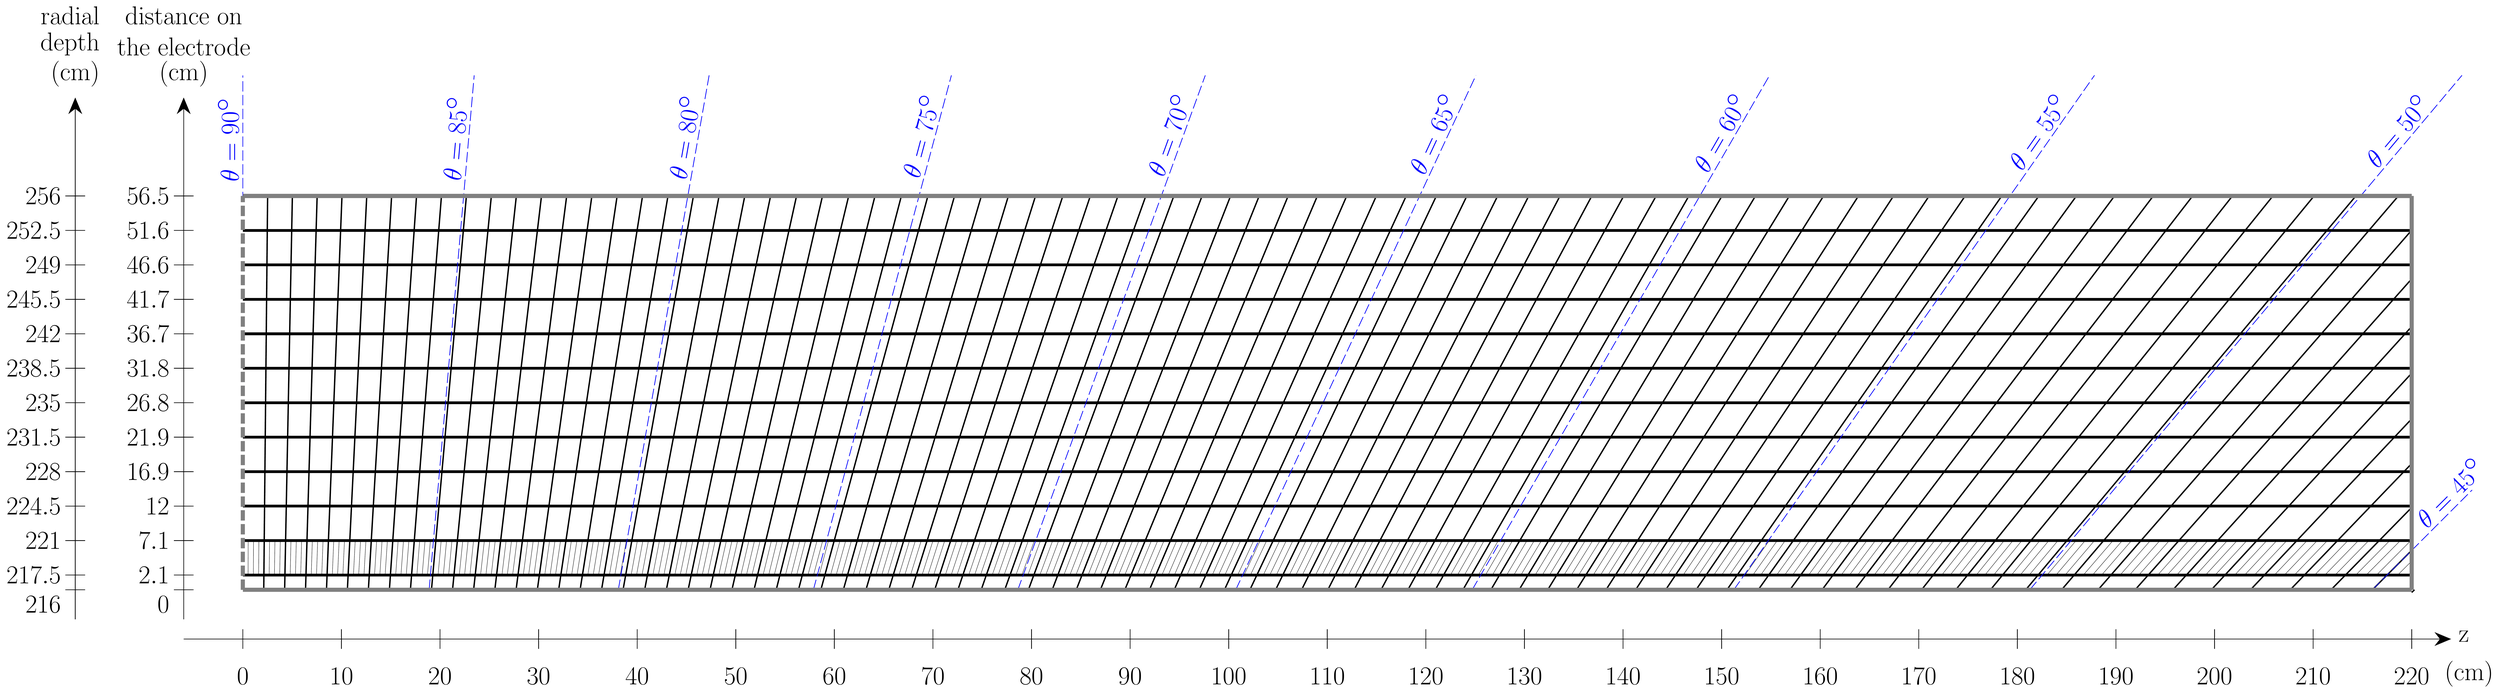
\begin{tikzpicture}[xscale=1,yscale=1,line/.style={<->,shorten >=0.4cm,shorten <=0.4cm},thick]\footnotesize
 \pgfmathsetmacro{\xone}{0}
 \pgfmathsetmacro{\xtwo}{220} % z at which the calo ends
 \pgfmathsetmacro{\yone}{216} % radius at which the calo starts
 \pgfmathsetmacro{\ytwo}{{\yone+40}}
 \pgfmathsetmacro{\ytwoNotProjected}{{\yone+56.5}}
 \def\drFirst{1.5}
 \def\drRest{3.5}
 \def\drFirstNotProjected{2.118615}
 \def\drRestNotProjected{4.943434}
 \def\ratio{1}


 % yaxis length parallel to the readout
\begin{scope}[line width = 2pt,  black,font={\fontsize{50pt}{12}\selectfont}]<+->;
  % vertical line
  \draw[-{Stealth[scale=4,width=10pt]}] (\xone - 6,\yone - 3) -- coordinate (y axis mid) (\xone - 6,\ytwo + 10 * \ratio) node [above,  yshift=200pt, scale = 3,xshift=0pt] {distance on}  node [above,  yshift=110pt, scale = 3,xshift=0pt] {the electrode} node [above, yshift=20pt,scale = 3] {(cm)};
  % first tick
  \foreach \y in {0}
  \draw (\xone - 7, {\yone + \y}) -- (\xone - 5,{\yone + \y}) node[left, midway, xshift = -30, yshift = -42, scale = 3] {\pgfmathparse{\y} \pgfmathprintnumber[fixed, precision = 0]{\pgfmathresult}};
  % all the other ticks
  \foreach \y in {0,...,11}
  \draw (\xone - 7, {\yone + \drFirst + \y * \drRest}) -- (\xone - 5,{\yone + \drFirst + \y * \drRest}) node[left, midway, xshift = -30, scale = 3] {\pgfmathparse{\drFirstNotProjected + \y*\drRestNotProjected} \pgfmathprintnumber[fixed,precision=1]{\pgfmathresult}};
\end{scope}

% yaxis depth projected readout (radial depth)
\begin{scope}[line width = 2pt,  black, font={\fontsize{50pt}{12}\selectfont}]<+->;
  % vertical line
  \draw[-{Stealth[scale = 4, width = 10pt]}] (\xone - 17,\yone - 3) -- coordinate (y axis mid) (\xone - 17,\ytwo + 10 * \ratio) node [above,  yshift = 200pt, scale = 3, xshift = -5pt] {radial} node [above, yshift = 110pt, scale = 3, xshift=-5pt] {depth} node [above, yshift = 20pt, scale = 3] {(cm)};
  \foreach \y in {0}
  \draw (\xone - 18, {\yone + \y}) -- (\xone - 16,{\yone + \y}) node[left, midway, xshift = -30, yshift = -42, scale = 3] {\pgfmathparse{\yone} \pgfmathprintnumber[fixed, precision = 0]{\pgfmathresult}};
  \foreach \y in {0,...,11}
  \draw (\xone - 18, {\yone + \drFirst + \y * \drRest}) -- (\xone - 16,{\yone + \drFirst + \y * \drRest}) node[left, midway, xshift =- 30, scale=3] {\pgfmathparse{\yone+ \drFirst  + \y*\drRest} \pgfmathprintnumber[fixed,precision=1]{\pgfmathresult}};
\end{scope}

% x axis
\begin{scope}[line width = 2pt,  black,font={\fontsize{50pt}{12}\selectfont}]<+->;
    % horizontal line
  \draw[-{Stealth[scale=4,width=10pt]}] (\xone - 6, \yone - 5) -- coordinate (y axis mid) (\xtwo + 4, \yone - 5) node [right, xshift=10pt, yshift=8pt, scale = 3] {z} node [right, xshift=-30pt, yshift=-100pt, scale = 3] {(cm)};
  \foreach \z in {0,...,22}{
  \pgfmathsetmacro{\realdistfromzero}{\z*10}
  \draw ({\xone + 10*\z},\yone - 6) --  (\xone  + 10*\z, \yone - 4) node[below, yshift = - 100pt, scale=3] {\pgfmathprintnumber[fixed,precision=0]{\realdistfromzero}};
  }
\end{scope}

% Draw all the diagonal lines separately for the strip layer and regular cells (one line per theta cell goes accross all layers for longitudinal cells)
\begin{scope}[very thick, black, line width = 1pt]
\pgfmathsetmacro{\dtheta}{0.5625/4.0}
\foreach \x in {1, ..., 319}
% the one from strip layer that do not have to be cut
\draw ({(\yone+\drFirst)*tan(\x * \dtheta))}, \yone+\drFirst) -- ({(\yone+\drFirst+\drRest) * tan(\x * \dtheta)}, \yone+\drFirst+\drRest);
% the one from strip  layer that need to be cut because close to the edge
\foreach \x in {320,..., 322}
\draw ({(\yone+\drFirst)*tan(\x * \dtheta))}, \yone+\drFirst) -- (\xtwo,{\xtwo*tan(90 - \x * \dtheta)});
\end{scope}
\begin{scope}[very thick, black, line width = 4pt]
\def\dtheta{0.5625}
\foreach \x in {1, ..., 72}
% the diagonal line from regular cells that do not need to be cut
\draw ({\yone*tan(\x * \dtheta))}, \yone) -- ({\ytwo * tan(\x * \dtheta)}, \ytwo);
\foreach \x in {73,..., 81}
% the diagonal line from regular cells that need to be cut
\draw ({\yone*tan(\x * \dtheta))}, \yone) -- (\xtwo, {\xtwo * tan(90 - \x * \dtheta)});
\end{scope}
% horizontal lines separating the layers
\begin{scope}[very thick, black, line width = 8pt]
\foreach \layer in {1,...,1}%pre sampler
\draw (\xone,\yone+\layer*\drFirst) -- (\xtwo, \yone+\layer*\drFirst);
\foreach \layer in {1,...,11}
\draw (\xone,\yone+\drFirst+\layer*\drRest) -- (\xtwo, \yone+\drFirst+\layer*\drRest);
\end{scope}

% Draw the blue lines showing theta values (not linked to the cell delta theta, just to print some reference)
\begin{scope}[line width = 2pt,  dashed,dash pattern=on 30pt off 10pt, blue,font={\fontsize{50pt}{12}\selectfont}]<+->;
   \def\dtheta{5}
   \def\drend{\drRest*3.5}
   % the one that do not need to be cut
   \foreach \x in {0,..., 8}
   \draw ({\yone*tan(\x * \dtheta))}, \yone) -- ({(\ytwo + \drend) * tan(\x * \dtheta)}, \ytwo + \drend) node [above, very near end, scale=3, rotate = {90 - \x * \dtheta} ] {$\theta$ = \pgfmathparse{90 - \x * \dtheta} \pgfmathprintnumber[fixed,precision=1]{\pgfmathresult}$^\circ$};
   \pgfmathsetmacro{\xend}{(\ytwo+\drend*1.1) * tan( 8 * \dtheta)}
   % the one that need to be cut because close to the edge
   \foreach \x in {9,..., 9}
   \draw ({\yone*tan(\x * \dtheta))}, \yone) -- (\xend, {\xend * tan(90 - \x * \dtheta)}) node [above, very near end, scale=3, rotate = {90 - \x * \dtheta} ] {$\theta$ = \pgfmathparse{90-\x*\dtheta} \pgfmathprintnumber[fixed,precision=1]{\pgfmathresult}$^\circ$};
 \end{scope}

% Draw the outer lines surrounding all the cells
\begin{scope}[line width = 12pt, black]<+->;
  \draw[gray,-] (\xone, \yone) -- (\xtwo, \yone) {};
  \draw[gray,-] (\xone, \ytwo) -- (\xtwo, \ytwo) {};
  \draw[gray,-,dashed,dash pattern=on 30pt off 10pt] (\xone, \yone) -- (\xone, \ytwo) {};
  \draw[gray,-] (\xtwo, \yone) -- (\xtwo, \ytwo) {};
\end{scope}

\end{tikzpicture}

\end{document}
